\section{Multichannel Cross-Layer Routing Protocol}
\label{sec:multichannel}

Our Multichannel Cross-Layer Routing Protocol (MCRP) concentrates on finding channels for nodes that are
free from or have low interference.  It allows the allocation of these channels in a way likely
to minimise the chances of nodes which are physically near communicating on the same channel and
hence reduce cross interference between different pairs of nodes.

\subsection{Overview}

%\explain the ideas (state machine?), reasons for doing

The design of the multichannel protocol is based on several crucial observations:
\begin{itemize}
\item Channel assignment - Sensors have limited memory and battery capabilities. In order to maximise the sensors lifetime, a centralised LPBR that has larger memory and fully powered is used for decision making. LPBR has a complete knowledge of the topology which enables it to make good channel assignment decisions based on the criteria that are explained in the next section. 
%LPBR assigns channel to the nodes.
%This centralised processes at the LPBR enable the other nodes that are battery powered to minimise the use of the energy in packets transmission. LPBR is fully powered which is the main reason for placing intelligence on it.
%LPBR keeps track of the channel conditions based on the feedback it receives from the nodes. All intelligence is done at LPBR.
%by considering load balancing in channels.
\item Interference - External interference cannot be predicted, thus channels cannot be allocated beforehand as it varies over time and locations. It is impossible to determine a single channel that is free from interference at any location. Our protocol checks the channel condition each time before deciding on a channel change to reduce interference and maximise throughput.
\item Frequency diversity - RPL is typically used with ContikiMAC which is a single channel protocol. By using multichannel, we increase the robustness of the network towards interference. However, applying multichannel to the existing RPL may hinder neighbour detection and RPL processes to maintain the network topology as it does not switch to the correct channel. We overcome this problem by enabling unicast in neighbour detection and RPL control messages. %We assume that no new nodes should join the topology after the initial setup.
%we need to ensure the node knows the correct channel to reach the neighbours. RPL forms and maintains the network topology through its control messages. Applying multichannel to the existing RPL may hinder neighbour detection and RPL processes and it does not have any means of switching to the correct channel. 
\end{itemize}

Our cross-layer multi-channel protocol focuses on the network and application layer of the protocol. This allows channel assignment decisions to be made thoroughly without being limited by the low layer complexity. The channel assignment processes take place only after the topology tree has been formed by RPL and stabilised.  The system
has two parts: a central algorithm which can be colocated with the LPBR and selects which channel each node should listen on; and a protocol which allows the network to communicate the channel change decision, probe the new channel and either communicate the success of the change or fall back to the previous channel. 

%Figure 1 shows the design of Multichannel RPL. The states are explained in the next sections.

%\begin{figure}
%\centering
%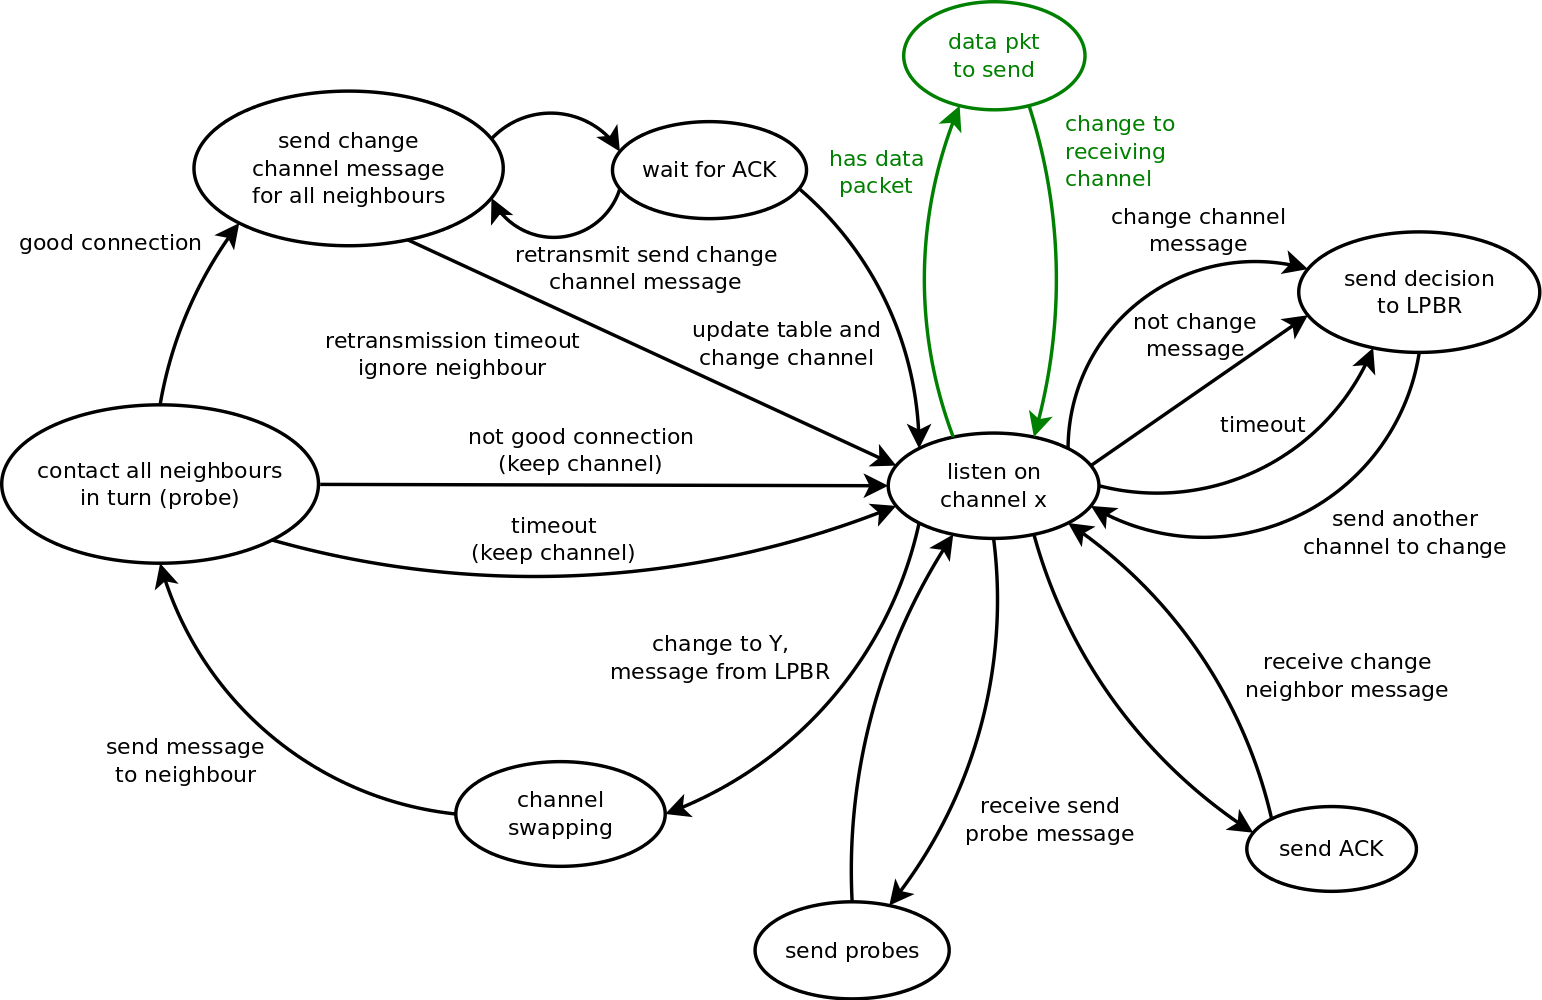
\includegraphics[height=7.2cm]{stateDiagram}
%\caption{State machine for channel switching.}
%\label{fig:example}
%\end{figure}

\subsection{Channel Selection Strategy}

%//LPBR decides the channel; random at first (or maybe not) and then based on probing that were done previously stating the condition of channels.
%//be more detail - better description of 2-hop strategy reasoning. %WHY?? keep them not to interference so much with each other
The system we propose is general and any algorithm can be used at the LPBR to assign channels.  In this paper we
use a two-hop colouring protocol to select a channel to be assigned to a node.  Channels are chosen in a way that
ensures no nodes within two hops of each other on the network are listening on the same channel.
This allows fair load balancing on the channels and reduces channel interference that could occur when two nearby nodes transmit together on the same channel. The nodes used in this paper have a transmission range of approximately 50 metres indoors and 125 metres outdoors.  It could be the case, therefore, that many nodes in a sensor network are in the transmission range of each other and potentially interfered with.

As in standard RPL all nodes are initialised to channel 26 by default.  The usual RPL set up mechanism is used to exchange control messages that are required to form an optimised topology before channel assignments can take place. The nodes will only be on the same channel once during the initial setup. Channel 26 is chosen as this is the usual RPL default initial channel since it often has fewer interference problems with WiFi and other sources. The studies in \cite{chrysso}\cite{micmac}\cite{watteyne} use several channels in their experiments and have channel 26 in common.
	
%**TWO HOP COLOURING STRATEGY?
%\subsubsection{Two Hops Neighbour Strategy -}


%//how it works?
%During the initial setup, LPBR does not have any knowledge of the channels condition. All channels are assumed to be available to be used. LPBR assigns a random channel to a node. The node that receives the channel change message will inform all of its neighbour of its new channel. The neighbours will update their neighbour table to hold the new channel value as the node current channel for transmission. The neighbour nodes will in turn, send probing messages.

\iffalse
\begin{algorithm}
\caption{Two hops neighbour strategy}
\begin{algorithmic} 
\STATE $newChannel \neq currentChannel$
\STATE $newChannel \leftarrow x$

\REQUIRE\emph{first hop}{}:
\WHILE {$retry \neq 4$}
\IF{$node = LPBRneighbour$}

\IF {$newChannel \neq LPBRChannel$}
\STATE {\emph {second hop}}
\ELSE
\STATE $newChannel \leftarrow y$
\ENDIF

\ELSE [$node = neighbourNeighbour$]
\IF {$newChannel \neq neighbourChannel$}
\STATE {\emph {second hop}}
\ELSE
\STATE $newChannel \leftarrow y$
\ENDIF
\ENDIF
\ENDWHILE


\REQUIRE\emph{second hop}{}:
\WHILE {$retry \neq 4$}
\IF{$node = LPBRneighbour$}

\IF {$newChannel \neq LPBRneighboursChannel$}
\STATE $newChannel \leftarrow OK$
\ELSE
\STATE $newChannel \leftarrow y$
\ENDIF

\ELSE [$node = neighbourNeighbour$]
\IF {$newChannel \neq neighbourNeighboursChannel$}
\STATE $newChannel \leftarrow OK$
\ELSE
\STATE $newChannel \leftarrow y$
\ENDIF
\ENDIF
\ENDWHILE
\end{algorithmic}
\end{algorithm}
\fi

In the two-hop colouring algorithm, the LPBR chooses a node to which it will assign a channel to listen on.  
This selection is random from channels 11 to 26 (the full range available).  The algorithm checks neighbours and neighbours of neighbours to see if any of those are listening on this channel already.  If any are a new channel is picked from the remaining list of available channels.  If the LPBR has knowledge of existing bad channels then those channels can be black listed.  Knowledge of channel interference (gained by probing, see later description) can be used to decide that a channel should not be used.  If a channel is found then the channel switching protocol is used (see section \ref{sec:channelswitch}).  If no channel can be found meeting these conditions the current
channel is kept.  

The node selection algorithm must only attempt one channel change at a time.  The protocol ensures that the
channel change attempt will always result in a message returned to the LPBR either confirming the new channel
or announcing a reversion to the old channel.  Until one or other of these happens no new channel change will
be made.

%***probing tries to avoid the interference channel.


%We could increase the number of probing messages by increasing the buffer size or the radio duty cycle (to be confirmed!!) but we chosen not to because increasing buffer size means that we will be using more memory which is not practical as we have limited memory available. If we increase the radio duty cycle, that would cost us more energy as the node will be awake more frequent and the nodes will not be in sync as they would have different radio duty cycle. That would increase the chance of packet loss. Our other option is to run the probing for a longer time.

%////FUTURE WORK?
%Even though external interference varies over time, it is unlikely that the channel quality fluctuates frequently within minutes that would affect the receiving success rate. Thus, the channel quality check is invoke on three (cases? situations?); on initialisation, when receiving LPBR channel change message and when the packet delivery ratio (PDR) drops. ***NOT SURE  


%****
%Each node keeps the counter of packets it has sent and received. It will send the information to LPBR periodically in order for LPBR to get a full view on the condition of the channels. LPBR will then decide if the node needs to change to another channel depending on the sent and received information. If the node does not perform well based on the number of received packets less than the number of packets being sent, LPBR will decide on a new channel the node needs to change into. The node will go through the channel changing processes to decide if the new channel is performing better than the previous channel before (settling?) for the new channel.

\subsection{Channel Switching}
\label{sec:channelswitch}

%//explain LPBR that decides whether the nodes should stay on the same channel or switch to a new channel based on the information it gathers through nodes probing.

%State machine explanation should be here?

\begin{figure}
\centering
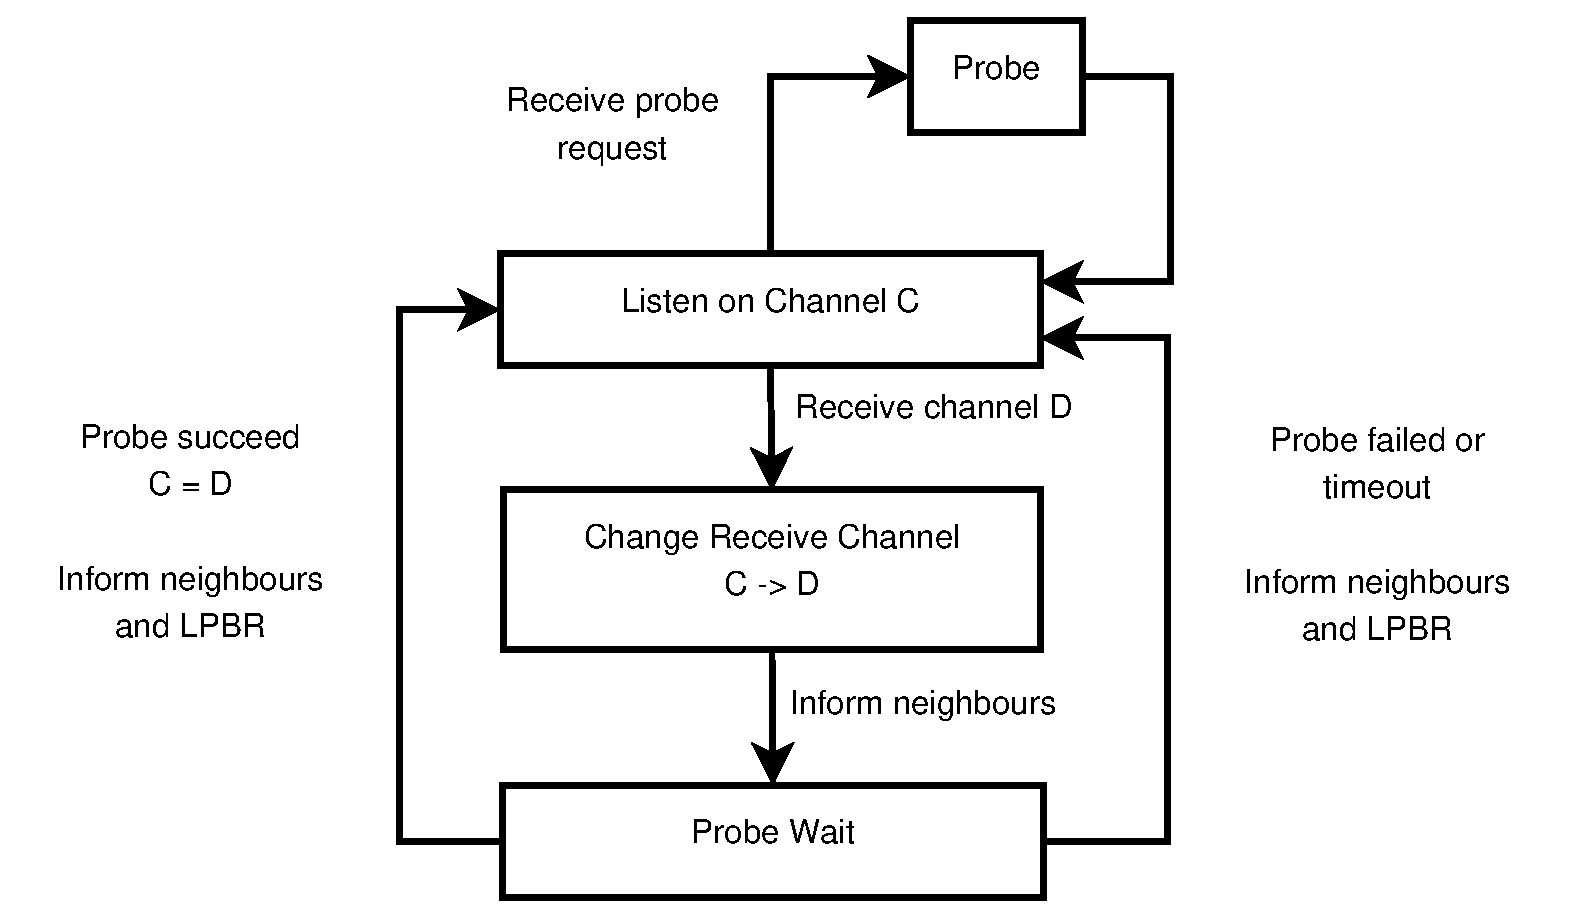
\includegraphics[width=3.5in]{Diagram1.eps}
\caption{Channel switching processes}
\label{fig_sim}
\end{figure}

Figure \ref{fig_sim} shows the state machine for the channel switching protocol.
As explained in the previous section, a choice of a new channel by the channel selction algorithm causes a change channel message to be sent to the appropriate node. 
On receiving a channel change message a node $N$ stores its current channel $C$ and communicates to all its neighbours the new channel $D$ it wishes to change to.  Those neighbours will update their neighbour tables to ensure that they now send to node $N$ on channel $D$.  The node $N$ now begins the channel quality checking process (see section \ref{sec:channelquality} with each neighbour in turn by sending them a probe request.  If this process fails for any neighbour then the node reverts to channel $C$.  Node $N$ informs its neighbours of this reversion to channel $C$ and informs the LPBR of the channel checking results and its reversion to listening on channel $C$.  If all channel quality checks succeed the node $N$.  It is important to emphasise that the network remains fully functional and connected at all stages of this protocol (however, the channel checking process uses probe packets that might interfere with other transmissions temporarily).

\subsection{Channel Quality Checking}
\label{sec:channelquality}
%channel quality check = probing
%//Channel condition is checked by probing before deciding to switch unless LPBR has the information regarding the specific channel based on probing that were done previously.

In describing the channel quality checking process it is worth emphasising the RPL distinction between neighbours and tree neighbours.  In RPL node neighbours are all nodes that a given node knows it could transmit to.  Tree neighbours are the nodes that a node does transmit to through the topology formed by the RPL protocol.

The channel quality checking is invoked each time a node changes channel after receiving a message from the LPBR.  A node $N$ changing to channel $D$ informs all neighbours in turn, of the new channel $D$ it will be listening on as described in the previous section.  It then enters the Probe Wait state and begins channel quality checking with each tree neighbour in turn.  

In the Probe Wait state node $N$ sends a Probe message to each neighbour in turn.  That neighbour will respond
to the message by sending eight packets to $N$ on the new channel $D$.  If this process times out (because of some communication failure) or the number of probe packets received is below a threshold (currently set to
seven) then node $N$ immediately exits Probe Wait, does not request more probes and reverts to channel $C$ its
previous channel.  All neighbours are informed of the change back to channel $C$ and the LPBR is informed of
the quality check failure with a summary of all probes received.
If, on the other hand, all channel quality checks succeed the change to channel $D$ becomes permanent for node $N$ and it informs the LPBR of the results of the probing (numbers of packets received) and the channel change.

Probing is an important part in making the channel change decision. It gives a quick overview of the channel condition based on the number of probing messages received. It is worth noting that probing is only done between the node and the tree neighbours. Neighbours that are not tree neighbours will not use the node as a route during their transmission thus there is no need for probing to take place with those neighbours. However, the neighbours still need to know the channel value as RPL control messages are sent to neighbours directly without using the routes.

%It is possible that the node itself ask for a channel change if its PDR is below a threshold. LPBR checks and updates the information of the channels and sends a change channel message. The steps as previously explained are repeated. ***NOT SURE? LPBR asks for the transmission and receiver rate periodically from all the nodes to decide a channel change.

%LPBR sends a change channel message after ***some time to check the condition of the node's channel and to get updates on the channels. The node's neighbours will start probing on the channel which the result is use to decide the changes.

%\subsection{LPBR Strategies}   
